\documentclass[border=2pt]{standalone}
\usepackage{tikz}
\usetikzlibrary{arrows.meta}

% Brand color definitions (RGB 0-1 scale)
\definecolor{Garnet}{rgb}{0.451, 0.0, 0.039}
\definecolor{Atlantic}{rgb}{0.275, 0.416, 0.624}
\definecolor{Congaree}{rgb}{0.122, 0.255, 0.302}
\definecolor{Horseshoe}{rgb}{0.396, 0.471, 0.043}
\definecolor{Rose}{rgb}{0.8, 0.18, 0.251}
\definecolor{Honeycomb}{rgb}{0.643, 0.569, 0.216}
\definecolor{Grass}{rgb}{0.0, 0.8, 0.0}
\definecolor{Black90}{rgb}{0.212, 0.212, 0.212}
\definecolor{Black70}{rgb}{0.361, 0.361, 0.361}
\definecolor{Black50}{rgb}{0.635, 0.635, 0.635}

% Gradient trail colors for Panel 3 (age index 1=newest, 8=oldest)
% Interpolation: green -> Honeycomb -> Rose as age increases
% age 1 (newest):  near Grass
% age 3:           Grass->Honeycomb blend
% age 5:           Honeycomb
% age 7:           Honeycomb->Rose blend
% age 8 (oldest):  Rose
\definecolor{Grad1}{rgb}{0.0, 0.8, 0.0}          % Green (newest)
\definecolor{Grad2}{rgb}{0.32, 0.68, 0.11}       % Green->Honeycomb 33%
\definecolor{Grad3}{rgb}{0.643, 0.569, 0.216}   % Honeycomb (50%)
\definecolor{Grad4}{rgb}{0.643, 0.569, 0.216}   % Honeycomb
\definecolor{Grad5}{rgb}{0.722, 0.375, 0.234}   % Honeycomb->Rose 67%
\definecolor{Grad6}{rgb}{0.800, 0.180, 0.251}   % Rose (~83%)
\definecolor{Grad7}{rgb}{0.800, 0.180, 0.251}   % Rose
\definecolor{Grad8}{rgb}{0.800, 0.180, 0.251}   % Rose (oldest)

\begin{document}

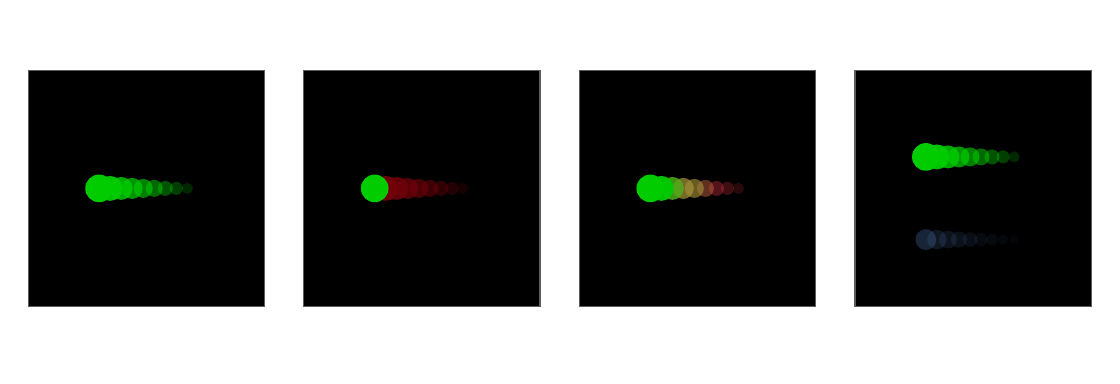
\begin{tikzpicture}[font=\sffamily]

  % Panel width = 3cm, gap = 0.5cm
  % Target moves LEFT -> trail extends to the RIGHT of current position
  % Current target dot at x=0.90cm, trail dots packed closer together
  % Trail dot x-positions (8 trail dots, step=0.14cm):
  %   dot 1 (newest) at x=1.04, dot 8 (oldest) at x=2.02
  %   x values: 1.04, 1.18, 1.32, 1.46, 1.60, 1.74, 1.88, 2.02
  % Current target at x=0.90, y=1.50
  % Dot sizes scaled ~2.5x: current=5pt, trail newest=4.5pt, oldest=2.0pt
  %   size step = (4.5 - 2.0)/7 = 0.357pt
  %   age1=4.50pt, age2=4.14pt, age3=3.79pt, age4=3.43pt,
  %   age5=3.07pt, age6=2.71pt, age7=2.36pt, age8=2.00pt
  % opacity (monochrome/proportional): newest=0.95, oldest=0.20, step=0.107

  % -------------------------------------------------------
  % PANEL 1: Monochrome
  % -------------------------------------------------------
  \begin{scope}[xshift=0cm]
    \fill[black] (0,0) rectangle (3.0,3.0);

    % Title above panel
    \node[white, anchor=south] at (1.5, 3.05)
      {\footnotesize\textbf{Monochrome}};

    % Trail dots (Grass, opacity decays with age)
    % age 8 (oldest, rightmost)
    \fill[Grass, opacity=0.20] (2.02, 1.50) circle (2.00pt);
    \fill[Grass, opacity=0.31] (1.88, 1.50) circle (2.36pt);
    \fill[Grass, opacity=0.41] (1.74, 1.50) circle (2.71pt);
    \fill[Grass, opacity=0.52] (1.60, 1.50) circle (3.07pt);
    \fill[Grass, opacity=0.63] (1.46, 1.50) circle (3.43pt);
    \fill[Grass, opacity=0.73] (1.32, 1.50) circle (3.79pt);
    \fill[Grass, opacity=0.84] (1.18, 1.50) circle (4.14pt);
    \fill[Grass, opacity=0.95] (1.04, 1.50) circle (4.50pt);  % age 1 (newest)
    % Current target
    \fill[Grass] (0.90, 1.50) circle (5pt);

    \draw[Black70, line width=0.4pt] (0,0) rectangle (3.0,3.0);

    % Panel label below
    \node[white, anchor=north] at (1.5, -0.10) {\footnotesize (a)};
  \end{scope}

  % -------------------------------------------------------
  % PANEL 2: Two-tone
  % -------------------------------------------------------
  \begin{scope}[xshift=3.5cm]
    \fill[black] (0,0) rectangle (3.0,3.0);

    \node[white, anchor=south] at (1.5, 3.05)
      {\footnotesize\textbf{Two-tone}};

    % All trail dots in Garnet (dark red), opacity decays with age
    \fill[Garnet, opacity=0.20] (2.02, 1.50) circle (2.00pt);
    \fill[Garnet, opacity=0.31] (1.88, 1.50) circle (2.36pt);
    \fill[Garnet, opacity=0.41] (1.74, 1.50) circle (2.71pt);
    \fill[Garnet, opacity=0.52] (1.60, 1.50) circle (3.07pt);
    \fill[Garnet, opacity=0.63] (1.46, 1.50) circle (3.43pt);
    \fill[Garnet, opacity=0.73] (1.32, 1.50) circle (3.79pt);
    \fill[Garnet, opacity=0.84] (1.18, 1.50) circle (4.14pt);
    \fill[Garnet, opacity=0.95] (1.04, 1.50) circle (4.50pt);
    % Current target: bright Grass
    \fill[Grass] (0.90, 1.50) circle (5pt);

    \draw[Black70, line width=0.4pt] (0,0) rectangle (3.0,3.0);
    \node[white, anchor=north] at (1.5, -0.10) {\footnotesize (b)};
  \end{scope}

  % -------------------------------------------------------
  % PANEL 3: Gradient
  % -------------------------------------------------------
  \begin{scope}[xshift=7.0cm]
    \fill[black] (0,0) rectangle (3.0,3.0);

    \node[white, anchor=south] at (1.5, 3.05)
      {\footnotesize\textbf{Gradient}};

    % Trail: green (newest) -> Honeycomb -> Rose (oldest)
    % Opacity also decays with age
    \fill[Grad8, opacity=0.20] (2.02, 1.50) circle (2.00pt);  % oldest, Rose
    \fill[Grad7, opacity=0.31] (1.88, 1.50) circle (2.36pt);
    \fill[Grad6, opacity=0.41] (1.74, 1.50) circle (2.71pt);
    \fill[Grad5, opacity=0.52] (1.60, 1.50) circle (3.07pt);
    \fill[Grad4, opacity=0.63] (1.46, 1.50) circle (3.43pt);
    \fill[Grad3, opacity=0.73] (1.32, 1.50) circle (3.79pt);
    \fill[Grad2, opacity=0.84] (1.18, 1.50) circle (4.14pt);
    \fill[Grad1, opacity=0.95] (1.04, 1.50) circle (4.50pt);  % newest, Grass
    % Current target: bright Grass
    \fill[Grass] (0.90, 1.50) circle (5pt);

    \draw[Black70, line width=0.4pt] (0,0) rectangle (3.0,3.0);
    \node[white, anchor=north] at (1.5, -0.10) {\footnotesize (c)};
  \end{scope}

  % -------------------------------------------------------
  % PANEL 4: Intensity-mapped
  % -------------------------------------------------------
  \begin{scope}[xshift=10.5cm]
    \fill[black] (0,0) rectangle (3.0,3.0);

    \node[white, anchor=south] at (1.5, 3.05)
      {\footnotesize\textbf{Intensity-mapped}};

    % Strong target (upper track, y=1.9): bright Grass trail
    \fill[Grass, opacity=0.20] (2.02, 1.90) circle (2.00pt);
    \fill[Grass, opacity=0.31] (1.88, 1.90) circle (2.36pt);
    \fill[Grass, opacity=0.41] (1.74, 1.90) circle (2.71pt);
    \fill[Grass, opacity=0.52] (1.60, 1.90) circle (3.07pt);
    \fill[Grass, opacity=0.63] (1.46, 1.90) circle (3.43pt);
    \fill[Grass, opacity=0.73] (1.32, 1.90) circle (3.79pt);
    \fill[Grass, opacity=0.84] (1.18, 1.90) circle (4.14pt);
    \fill[Grass, opacity=0.95] (1.04, 1.90) circle (4.50pt);
    % Strong target current dot
    \fill[Grass] (0.90, 1.90) circle (5pt);

    % Weak target (lower track, y=0.85): Atlantic (blue-tinted), low opacity
    % Dot sizes scaled ~2.5x from 0.6-1.5pt range -> 1.50-3.50pt range
    %   size step = (3.5 - 1.5)/7 = 0.286pt
    %   age1=3.50pt, age2=3.21pt, age3=2.93pt, age4=2.64pt,
    %   age5=2.36pt, age6=2.07pt, age7=1.79pt, age8=1.50pt
    % Base opacity = 0.22, further scaled by age decay (newest=0.22, oldest=0.05)
    \fill[Atlantic, opacity=0.05] (2.02, 0.85) circle (1.50pt);
    \fill[Atlantic, opacity=0.07] (1.88, 0.85) circle (1.79pt);
    \fill[Atlantic, opacity=0.09] (1.74, 0.85) circle (2.07pt);
    \fill[Atlantic, opacity=0.11] (1.60, 0.85) circle (2.36pt);
    \fill[Atlantic, opacity=0.14] (1.46, 0.85) circle (2.64pt);
    \fill[Atlantic, opacity=0.16] (1.32, 0.85) circle (2.93pt);
    \fill[Atlantic, opacity=0.19] (1.18, 0.85) circle (3.21pt);
    \fill[Atlantic, opacity=0.22] (1.04, 0.85) circle (3.50pt);
    % Weak target current dot (dim blue)
    \fill[Atlantic, opacity=0.35] (0.90, 0.85) circle (3.75pt);

    \draw[Black70, line width=0.4pt] (0,0) rectangle (3.0,3.0);
    \node[white, anchor=north] at (1.5, -0.10) {\footnotesize (d)};
  \end{scope}

\end{tikzpicture}

\end{document}
